\mysectionlabel{Overview on \codeName }{sec:overview}
%
This section provides a general overview on important parts of \codeName\ . It is recommended to read these parts as it alleviates your life in creating models, understanding the behavior of the system and resolving errors.
%
\mysubsectionlabel{Module structure}{sec:overview:modulestructure}
This section will show:
\bi
  \item Overview of modules
  \item Conventions: dimension of nodes, objects and vectors
  \item Coordinates: reference coordinates and displacements
  \item Nodes, Objects, Markers and Loads
\ei
For an introduction to the solvers, see \refSection{sec:solvers}.
\onlyRST{

.. _fig-exudyn-candpython:
.. figure:: docs/theDoc/figures/overviewExudynModules.png
   :width: 350

   Overview on Exudyn C++ and Python modules

}

\begin{figure}
  \centering
  \begin{tikzpicture}[node distance = 2cm, auto]
      % Place nodes
      \node [cloud] (exu) {exudyn};
      \node [wideblock, above of=exu, xshift = 1cm] (exudynCPP) {\mybold{exudynCPP}: C++ module};
      \node [wideblock, below of=exu, xshift = 1cm] (exudynPython) {exudyn Python modules};
      \node [wideblock, right of=exudynPython, node distance=6cm, text width=5cm] (utilities) {\mybold{utilities}};
      \node [wideblock, below of=utilities, text width=5cm] (solvers) {\mybold{solvers}: interface to C++ solvers};
      \node [wideblock, below of=solvers, text width=5cm] (itemInterface) {\mybold{itemInterface}: main interface to C++ items};
      \node [wideblock, below of=itemInterface, text width=5cm] (FEM) {\mybold{FEM}: FEM import and preprocessing};
      \node [wideblock, below of=FEM, text width=5cm] (plot) {\mybold{plot}: interface to matplotlib};
      \node [wideblock, below of=plot, text width=5cm] (processing) {\mybold{processing}: parallelization and optimization};
      \node [wideblock, below of=processing, text width=5cm] (robotics) {\mybold{robotics} submodule};
      \node [wideblock, below of=robotics, text width=5cm] (etc) {...};

      % Draw edges
      \path [line] (exu) -- (exudynCPP);
      \path [line] (exu) -- (exudynPython);

      \path [line] (exudynPython) |- (itemInterface);
      \path [line] (exudynPython) |- (solvers);
      \path [line] (exudynPython) |- (utilities);
      \path [line] (exudynPython) |- (FEM);
      \path [line] (exudynPython) |- (plot);
      \path [line] (exudynPython) |- (processing);
      \path [line] (exudynPython) |- (robotics);
      \path [line] (exudynPython) |- (etc);
  \end{tikzpicture}
  \caption{Overview of exudyn C++ and Python modules.}
  \label{fig_exudyn_CandPython}
\end{figure}

\mysubsubsectionlabel{Overview of modules}{sec:overview:overviewmodules}
Currently, the \codeName\ module structure is split into a C++ core part and a set of 
Python parts, see \fig{fig_exudyn_CandPython}.
\bi
  \item \mybold{C++ parts}, see \fig{fig_exudyn_CPP} and \fig{fig_system_overview}:
  \bi
    \item[--] \texttt{exudyn}:
    on this level, there are just very few functions: \texttt{SystemContainer()}, \texttt{StartRenderer()}, \texttt{StopRenderer()}, \texttt{GetVersionString()}, \texttt{SolveStatic(...)}, \texttt{SolveDynamic(...)}, ... as well as system and user variable dictionaries \texttt{exudyn.variables} and \texttt{exudyn.sys}
    \item[--] \texttt{SystemContainer}: contains the systems (most important), solvers (static, dynamics, ...), visualization settings
    \item[--] \texttt{mbs}: \acf{mbs} created with \texttt{mbs = SC.AddSystem()}, this structure contains everything that defines a solvable multibody system; a large set of nodes, objects, markers, 
    loads can added to the system, see \refSection{sec:item:reference:manual};
    \item[--] \texttt{mbs.systemData}: contains the initial, current, visualization, ... states of the system and holds the items, see \fig{fig_system_overview}
  \ei
  \item \mybold{Python parts} (this list is continuously extended, see \refSection{sec:pythonUtilityFunctions}), sorted by importance:
  \bi
    \item[--] \texttt{exudyn.utilities}: constains helper classes in Python and includes \codeName\ modules \texttt{basicUtilities}, \texttt{rigidBodyUtilities}, \texttt{graphicsDataUtilities}, and \texttt{itemInterface}, which is recommended to be loaded at beginning of your model file
    \item[--] \texttt{exudyn.itemInterface}: contains the interface, which transfers Python classes (e.g., of a NodePoint) to dictionaries that can be understood by the C++ module
    \item[--] \texttt{exudyn.basicUtilities}: contains basic helper classes, without importing numpy
    \item[--] \texttt{exudyn.rigidBodyUtilities}: contains important helper classes for creation of rigid body inertia, rigid bodies, and rigid body joints; includes helper functions for rotation parameterization, rotation matrices, homogeneous transformations, etc.
    \item[--] \texttt{exudyn.graphicsDataUtilities}: provides some basic drawing utilities, definition of colors and basic drawing objects (including \acs{STL} import); rotation/translation of graphicsData objects
    \item[--] \texttt{exudyn.plot}: contains PlotSensor(...), a very versatile interface to matplotlib and other valuable helper functions
    \item[--] \texttt{exudyn.processing}: methods for optimization, parameter variation, sensitivity analysis, etc.
    \item[--] \texttt{exudyn.FEM}: everything related to finite element import and creation of model order reduction flexible bodies
    \item[--] \texttt{exudyn.robotics}: submodule containing several helper modules related to manipulators (\texttt{robotics}, \texttt{robotics.models}), mobile robots (\texttt{robotics.mobile}), trajectory generation (\texttt{robotics.motion}), etc.
    \item[--] \texttt{exudyn.beams}: helper functions for creation of beams along straight lines and curves, sliding joints, etc.
    \item[--] \texttt{exudyn.interactive}: helper classes to create interactive models (e.g. for teaching or demos)
    \item[--] \texttt{exudyn.physics}: containing helper functions, which are physics related such as friction
    \item[--] \texttt{exudyn.signalProcessing}: filters, FFT, etc.; interfaces to scipy and numpy methods
    \item[--] \texttt{exudyn.solver}: functions imported when loading \texttt{exudyn}, containing main solvers
  \ei
\ei
%
%++++++++++++++++++++++++++++++++++++++++++++++++++++++++++++++++++++++++
\onlyRST{

.. _fig-exudyn-cpp:
.. figure:: docs/theDoc/figures/overviewExudynCppModule.png
   :width: 500

   Overview on Exudyn C++ module

}
\begin{figure}
  \centering
  \begin{tikzpicture}[node distance = 2cm, auto]
      % Place nodes
      \node [cloud] (exu) {exudynCPP};
      \node [wideblock, below of=exu] (systemContainer) {SystemContainer};
      \node [wideblock, below of=systemContainer] (system) {MainSystem (e.g. 'mbs')};
      \node [wideblock, right of=systemContainer,  node distance=6cm] (visualizationSettings) {visualizationSettings};
      \node [block, below of=system] (systemData) {systemData};
      \node [wideblock, below of=systemData] (systemStates) {system states (initial, current, ...)};
      \node [wideblock, left of=systemContainer, node distance=6cm] (solver) {static and dynamic solver interfaces};
      \node [wideblock, below of=solver] (renderer) {basic renderer interface (start/stop)};
      \node [wideblock, below of=renderer] (misc) {data types, local dictionaries, system wide settings};
      
      \node [wideblock, dashed, fill=gray!10, right of=system,  node distance=6cm] (anotherSystem) {MainSystem (e.g. 'anotherMbs')};
      \node [block, dashed, fill=gray!10, below of=anotherSystem] (anotherSystemData) {systemData};
      \node [wideblock, dashed, fill=gray!10, below of=anotherSystemData] (anotherSystemStates) {system states 
      (initial, current, ...)};

      %\node [cloud, right of=exu] (itemInterface) {itemInterface.py};
      %\node [cloud, right of=itemInterface] (exudynUtilities) {exudynUtilities.py};

      % Draw edges
      \path [line] (exu) -- (systemContainer);
      \path [line] (systemContainer) -- (system);
      \path [line] (systemContainer) -- (visualizationSettings);
      \path [line] (system) -- (systemData);
      \path [line] (systemData) -- (systemStates);
      \path [line] (exu) -- (solver);
      \path [line] (solver) -- (renderer);
      \path [line] (renderer) -- (misc);

      \path [line, dashed] (systemContainer) -- (anotherSystem);
      \path [line, dashed] (anotherSystem) -- (anotherSystemData);
      \path [line, dashed] (anotherSystemData) -- (anotherSystemStates);
  \end{tikzpicture}
  \caption{Overview of exudyn C++ module.}
  \label{fig_exudyn_CPP}
\end{figure}
%++++++++++++++++++++++++++++++++++++++++++++++++++++++++++++++++++++++++

\onlyRST{

.. _fig-system-overview:
.. figure:: docs/theDoc/figures/overviewSystemData.png
   :width: 550

   Overview of systemData

SystemData connects items, states and stores the \acs{LTG}. Note that access to items is provided via functions in \texttt{MainSystem}.
}
%++++++++++++++++++++++++++++++++++++++++++++++++++++++++++++++++++++++++
\begin{figure}
  \centering
  \begin{tikzpicture}[node distance = 2cm, auto]
      % 
      \node [cloud] (system) {MainSystem ('mbs')};
      \node [wideblock, below of=system] (systemData) {systemData};
      \node [wideblock, left of=systemData, node distance=5cm] (systemStates) {system states};
      \node [wideblock, text width=3cm, below of=systemStates, xshift=-2cm] (current) {current state};
      \node [wideblock, text width=3cm, below of=current] (initial) {initial state};
      \node [wideblock, text width=3cm, below of=initial] (reference) {reference state};
      \node [wideblock, text width=3cm, dashed, fill=gray!10, below of=reference] (otherStates) {other states};
%
      \node [wideblock, right of=systemData, node distance=5cm] (ltg) {\acs{LTG} coordinate index lists};
%
      \node [wideblock, below of=systemData, xshift=2.4cm] (nodes) {list of nodes};
      \node [wideblock, below of=nodes] (objects) {list of objects};
      \node [wideblock, below of=objects] (markers) {list of markers};
      \node [wideblock, below of=markers] (loads) {list of loads};
      \node [wideblock, below of=loads] (sensors) {list of sensors};
%
      % Draw edges
      \path [line] (system) -- (systemData);
      \path [line] (systemData) -- (systemStates);
      \path [line] (systemStates) |- (current);
      \path [line] (systemStates) |- (initial);
      \path [line] (systemStates) |- (reference);
      \path [line, dashed] (systemStates) |- (otherStates);
%
      \path [line] (systemData) -- (ltg);
%
      \path [line] (systemData) |- (nodes);
      \path [line] (systemData) |- (objects);
      \path [line] (systemData) |- (markers);
      \path [line] (systemData) |- (loads);
      \path [line] (systemData) |- (sensors);
%
  \end{tikzpicture}
  \caption{Overview of systemData, which connects items, states and stores the \acs{LTG}. Note that access to items is provided via functions in \texttt{MainSystem}.}
  \label{fig_system_overview}

\end{figure}
%++++++++++++++++++++++++++++++++++++++++++++++++++++++++++++++++++++++++


\mysubsubsectionlabel{Conventions: items, indexes, coordinates}{sec:overview:conventionsitems}
In this documentation, we will use the term \mybold{item} to identify nodes, objects, markers, loads and sensors: \vspace{6pt}

  item $\in$ \{node, object, marker, load, sensor\} \vspace{12pt}

\noindent \mybold{Indexes: arrays and vectors starting with 0:} \vspace{6pt}\\
As known from Python, all \mybold{indexes} of arrays, vectors, matrices, ...\ are starting with 0. This means that the first component of the vector \texttt{v=[1,2,3]} is accessed with \texttt{v[0]} in Python (and also in the C++ part of \codeName ). The range is usually defined as \texttt{range(0,3)}, in which '3' marks the index after the last valid component of an array or vector.
\ignoreRST{\vspace{12pt}\\}
%
\mybold{Dimensionality of objects and vectors:} \ignoreRST{\vspace{6pt}}\\ 
\ac{2D} vs.\ \ac{3D}
\ignoreRST{\vspace{6pt}\\}
As a convention, quantities in \codeName\ are 3D, such as nodes, objects, markers, loads, measured quantities, etc. 
For that reason, we denote planar nodes, objects, etc.\ with the suffix 2D, but 3D objects do not get this suffix\footnote{There are some rare exceptions, such as Beam3D as the pure beam may easily lead to name space conflicts in Python}.

Output and input to objects, markers, loads, etc.\ is usually given by 3D vectors (or matrices), such as (local) position, force, torque, rotation, etc. However, initial and reference values for nodes depend on their dimensionality.
As an example, consider a \texttt{NodePoint2D}:
\bi
  \item \texttt{referenceCoordinates} is a 2D vector (but could be any dimension in general nodes)
  \item measuring the current position of \texttt{NodePoint2D} gives a 3D vector
  \item when attaching a \texttt{MarkerNodePosition} and a \texttt{LoadForceVector}, the force will be still a 3D vector
\ei
Furthermore, the local position in 2D objects is provided by a 3D vector. Usually, the dimensionality is given in the reference manual. User errors in the dimensionality will be usually detected either by the Python interface (i.e., at the time the item is created) or by the system-preprocessor

\mysubsectionlabel{Items: Nodes, Objects, Loads, Markers, Sensors, ...}{sec:overview:items}
%
In this section, the most important part of \codeName\ are provided. An overview of the interaction of the items is given in \fig{fig_items_interaction}

%++++++++++++++++++++++++++++++++++++++++++++++++++++++++++++++++++++++++
\onlyRST{

.. _fig-items-interaction:
.. figure:: docs/theDoc/figures/itemsMultibodySystem.png
   :width: 500

   Interaction of items in a multibody system

Note that both, bodies and connectors (including constraints) are -- computational -- objects. The arrows indicate, that, e.g., object 1 has node 1 and node 2 (indexes) and that marker 0 is attached to object 0, while load 0 uses marker 0 to apply the load. Sensors could additionally be attached to certain items.

}
%++++++++++++++++++++++++++++++++++++++++++++++++++++++++++++++++++++++++
\begin{figure}
  \centering
  \begin{tikzpicture}[node distance = 2cm, auto, thick,scale=0.7, every node/.style={scale=0.7}]
      % Place nodes
      \node [nodeBlock] (node0) {node 0};
      \node [nodeBlock, below of=node0, node distance=2cm] (node1) {node 1};
      \node [nodeBlock, below of=node1, node distance=2cm] (node2) {node 2};

      \node [objectBlock, right of=node0] (object0) {object 0 (body)};
      \node [objectBlock, right of=node1, yshift = -1cm] (object1) {object 1 (body)};
      
      \node [markerBlock, right of=object0] (marker0) {marker 0};
      \node [loadBlock, right of=marker0, node distance=3cm] (load0) {load 0};
      
      \node [markerBlock, left of=node2, yshift = -2cm, xshift = 1cm] (marker1) {marker 1};
      \node [markerBlock, right of=node2, yshift = -2cm] (marker2) {marker 2};

      \node [connectorBlock, below of=node2] (connector) {connector};


      \path [arrow] (object0) -- (node0);
      \path [arrow] (marker0) -- (object0);
      \path [arrow] (load0) -- (marker0);
      \path [arrow] (object1) -- (node1);
      \path [arrow] (object1) -- (node2);
      \path [arrow] (marker1) |- (node0);
      \path [arrow] (marker2) -- (object1);
      \path [arrow] (connector) -- (marker1);
      \path [arrow] (connector) -- (marker2);
      %\path [line] (systemData) |- (objects);
      %\path [line] (systemData) |- (markers);
      %\path [line] (systemData) |- (loads);

  \end{tikzpicture}
  \caption{Interaction of items in a multibody system. 
Note that both, bodies and connectors (including constraints) are -- computational -- objects.
The arrows indicate, that, e.g., object 1 has node 1 and node 2 (indexes) and that marker 0 is attached to object 0, while load 0 uses marker 0 to apply the load. Sensors could additionally be attached to certain items.}
  \label{fig_items_interaction}

\end{figure}
%++++++++++++++++++++++++++++++++++++++++++++++++++++++++++++++++++++++++

\mysubsubsection{Nodes}
Nodes provide the coordinates (and the degrees of freedom) to the system. They have no mass, stiffness or whatsoever assigned.
Without nodes, the system has no unknown coordinates.
Adding a node provides (for the system unknown) coordinates. In addition we also need equations for every nodal coordinate -- otherwise the system cannot be computed (NOTE: this is currently not checked by the preprocessor).

\mysubsubsection{Objects}
Objects are 'computational objects' and they provide equations to your system. Objects often provide derivatives and have measurable quantities (e.g. displacement) and they provide access, which can be used to apply, e.g., forces. Some of this functionality is only available in C++, but not in Python.

Objects can be a:
\bi
  \item general object (e.g.\ a controller, user defined object, ...; no example yet)
  \item body: has a mass or mass distribution; markers can be placed on bodies; loads can be applied; constraints can be attached via markers; bodies can be:
  \bi
    \item[--] ground object: has no nodes
    \item[--] simple body: has one node (e.g. mass point, rigid body)
    \item[--] finite element and more complicated body (e.g. FFRF-object): has more than one node
  \ei
  \item connector: uses markers to connect nodes and/or bodies; adds additional terms to system equations either based on stiffness/damping or with constraints (and Lagrange multipliers). Possible connectors:
  \bi
    \item[--] algebraic constraint (e.g. constrain two coordinates: $q_1 = q_2$)
    \item[--] classical joint
    \item[--] spring-damper or penalty constraint
  \ei
\ei

\mysubsubsection{Markers}
Markers are interfaces between objects/nodes and constraints/loads.
A constraint (which is also an object) or load cannot act directly on a node or object without a marker.
As a benefit, the constraint or load does not need to know whether it is applied, e.g., to a node or to a local position of a body.

Typical situations are:
\bi
  \item Node -- Marker -- Load
  \item Node -- Marker -- Constraint (object)
  \item Body(object) -- Marker -- Load
  \item Body1 -- Marker1 -- Joint(object) -- Marker2 -- Body2
\ei

\mysubsubsection{Loads}
Loads are used to apply forces and torques to the system. The load values are static values. However, you can use Python functionality to modify loads either by linearly increasing them during static computation or by using the 'mbs.SetPreStepUserFunction(...)' structure in order to modify loads in every integration step depending on time or on measured quantities (thus, creating a controller).

\mysubsubsection{Sensors}
Sensors are only used to measure output variables (values) in order to simpler generate the requested output quantities.
They have a very weak influence on the system, because they are only evaluated after certain solver steps as requested by the user.

\mysubsubsectionlabel{Reference coordinates and displacements}{sec:overview:items:coordinates}
Nodes usually have separated reference and initial quantities. Here, 
\texttt{referenceCoordinates} are the coordinates for which the system is defined upon creation. Reference coordinates are needed, e.g., for definition of joints and for the reference configuration of finite elements. In many cases it marks the undeformed configuration (e.g., with finite elements), but not, e.g., for \texttt{ObjectConnectorSpringDamper}, which has its own reference length. 

Initial displacement (or rotation) values are provided separately, in order to start a system from a configuration different from the reference configuration.
As an example, the initial configuration of a \texttt{NodePoint} is given by \texttt{referenceCoordinates + initialCoordinates}, while the initial state of a dynamic system additionally needs \texttt{initialVelocities}.

\mysubsectionlabel{Mapping between local and global coordinate indices}{sec:overview:ltgmapping}
%
The \ac{LTG}-index-mappings\footnote{local-to-global coordinate index mappings containing transformation from local object coordinate indices to global (system) coordinate indices; this is different for \mybold{coordinate transformations}!} between local coordinate \mybold{indices}, on node or object level, and global (=system) coordinate \mybold{indices} follows the following rules:
\bi
\item \ac{LTG}-index-mappings are computed during \texttt{mbs.Assemble()} and are not available before.
\item Nodes own a global index which relates the local coordinates to global (system) coordinate. E.g., for a \ac{ODE2} node with node number \texttt{i}, this index can be obtained via the function \texttt{mbs.GetNodeODE2Index(i)}.
\item The order of global coordinates is simply following the node numbering. If we add three nodes \texttt{NodePoint}, the system will contain 9 coordinates, where the first triple (starting index 0) belongs to node 0, the second triple (starting index 3) belongs to node 1 and the third triple (starting index 6) belongs to node 2. After \texttt{mbs.Assemble()}, you can access the system coordinates via \texttt{mbs.systemData.GetODE2Coordinates()}, which returns a numpy array with 9 coordinates, containing the initial values provided in \texttt{NodePoint} (default: zero).
\item Objects have their own \ac{LTG}-index-mappings for their respective coordinate types. The \ac{ODE2} coordinates of an object \texttt{j} can be retrieved via \texttt{mbs.systemData.GetObjectLTGODE2(j)}. For a body, these are the global \ac{ODE2} coordinates representing the body; for a connector, these are the coordinates to which the connector is linked (usually coordinates of two bodies); for a ground object, the \ac{LTG}-index-mapping is empty; see also \refSection{sec:systemData:ObjectLTG}.
\item Constraints create algebraic variables (Lagrange multipliers) automatically. For a constraint with object number \texttt{k}, the global index to algebraic variables (of \ac{AE}-type) can be accessed via \texttt{mbs.systemData.GetObjectLTGAE(k)}.
\ei

\mysubsectionlabel{Exudyn Basics}{sec:overview:basics}
This section will show:
\bi
  \item Interaction with the \codeName\ module
  \item Simulation settings
  \item Visualization settings
  \item Generating output and results
  \item Graphics pipeline
  \item Generating animations
\ei

\mysubsubsectionlabel{Interaction with the \codeName\ module}{sec:overview:basics:interactionmodule}
It is important that the \codeName\ module is basically a state machine, where you create items on the C++ side using the Python interface. This helps you to easily set up models using many other Python modules (numpy, sympy, matplotlib, ...) while the computation will be performed in the end on the C++ side in a very efficient manner. 
\vspace{12pt}\\
\mybold{Where do objects live?}\vspace{6pt}\\
%(where do objects live? state machine; graphics interaction)
Whenever a system container is created with \texttt{SC = exu.SystemContainer()}, the structure \texttt{SC} becomes a variable in the Python interpreter, but it is managed inside the C++ code and it can be modified via the Python interface.
Usually, the system container will hold at least one system, usually called \texttt{mbs}.
Commands such as \texttt{mbs.AddNode(...)} add objects to the system \texttt{mbs}. 
The system will be prepared for simulation by \texttt{mbs.Assemble()} and can be solved (e.g., using \texttt{exu.SolveDynamic(...)}) and evaluated hereafter using the results files.
Using \texttt{mbs.Reset()} will clear the system and allows to set up a new system. Items can be modified (\texttt{ModifyObject(...)}) after first initialization, even during simulation.
%

\mysubsubsectionlabel{Simulation settings}{sec:overview:basics:simulationsettings}
The simulation settings consists of a couple of substructures, e.g., for \texttt{solutionSettings}, \texttt{staticSolver}, \texttt{timeIntegration} as well as a couple of general options -- for details see \refSection{sec:SolutionSettings} and \refSection{sec:SimulationSettings}.

Simulation settings are needed for every solver. They contain solver-specific parameters (e.g., the way how load steps are applied), information on how solution files are written, and very specific control parameters, e.g., for the Newton solver. 

\noindent The simulation settings structure is created with 
\pythonstyle\begin{lstlisting}
  simulationSettings = exu.SimulationSettings()
\end{lstlisting}
%
Hereafter, values of the structure can be modified, e.g.,
\pythonstyle\begin{lstlisting}
  tEnd = 10 #10 seconds of simulation time:
  h = 0.01  #step size (gives 1000 steps)
  simulationSettings.timeIntegration.endTime = tEnd
  #steps for time integration must be integer:
  simulationSettings.timeIntegration.numberOfSteps = int(tEnd/h)
  #assigns a new tolerance for Newton's method:
  simulationSettings.timeIntegration.newton.relativeTolerance = 1e-9 
  #write some output while the solver is active (SLOWER):
  simulationSettings.timeIntegration.verboseMode = 2                 
  #write solution every 0.1 seconds:
  simulationSettings.solutionSettings.solutionWritePeriod = 0.1      
  #use sparse matrix storage and solver (package Eigen):
  simulationSettings.linearSolverType = exu.LinearSolverType.EigenSparse 
\end{lstlisting}

\mysubsubsection{Generating output and results}
%
The solvers provide a number of options in \texttt{solutionSettings} to generate a solution file. As a default, exporting the solution of all system coordinates (on position, velocity, ... level) to the solution file is activated with a writing period of 0.01 seconds.

\noindent Typical output settings are:
\pythonstyle\begin{lstlisting}
  #create a new simulationSettings structure:
  simulationSettings = exu.SimulationSettings()
  
  #activate writing to solution file:
  simulationSettings.solutionSettings.writeSolutionToFile = True
  #write results every 1ms:
  simulationSettings.solutionSettings.solutionWritePeriod = 0.001
  
  #assign new filename to solution file
  simulationSettings.solutionSettings.coordinatesSolutionFileName= "myOutput.txt"

  #do not export certain coordinates:
  simulationSettings.solutionSettings.exportDataCoordinates = False
\end{lstlisting}

Furthermore, you can use sensors to record particular information, e.g., the displacement of a body's local
position, forces or joint data. For viewing sensor results, use the \texttt{PlotSensor} function of the 
\texttt{exudyn.plot} tool, see the rigid body and joints tutorial.


\mysubsubsectionlabel{Visualization settings dialog}{sec:overview:basics:visualizationsettings}
%
Visualization settings are used for user interaction with the model. E.g., the nodes, markers, loads, etc., can be visualized for every model. There are default values, e.g., for the size of nodes, which may be inappropriate for your model. Therefore, you can adjust those parameters. In some cases, huge models require simpler graphics representation, in order not to slow down performance -- e.g., the number of faces to represent a cylinder should be small if there are 10000s of cylinders drawn. Even computation performance can be slowed down, if visualization takes lots of CPU power. However, visualization is performed in a separate thread, which usually does not influence the computation exhaustively.

Details on visualization settings and its substructures are provided in \refSection{sec:VSettingsGeneral} -- \refSection{sec:VisualizationSettings}. These settings may also be edited by pressing 'V' in the active render window (does not work, if there is no active render loop using, e.g., \texttt{SC.WaitForRenderEngineStopFlag()} or 
\texttt{mbs.WaitForUserToContinue()} ).
The visualization settings dialog is shown exemplarily in \fig{fig_visualizationSettings}.
Note that this dialog is automatically created and uses Python's \texttt{tkinter}, which is lightweight, but not very well suited if display scalings are large (e.g., on high resolution laptop screens). If working with Spyder, it is recommended to restart Spyder, if display scaling is changed, in order to adjust scaling not only for Spyder but also for \codeName\ .

The appearance of visualization settings dialogs may be adjusted by directly modifying \texttt{exudyn.GUI} variables (this may change in the future). For example write in your code before opening the render window\footnote{treeEdit and treeview both mean the settings dialog currently used for visualization settings and partially for right-mouse-click}:
\pythonstyle\begin{lstlisting}
  import exudyn.GUI
  exudyn.GUI.dialogDefaultWidth             #unscaled width of, e.g., right-mouse-button dialog
  exudyn.GUI.treeEditDefaultWidth = 800
  exudyn.GUI.treeEditDefaultHeight = 600
  exudyn.GUI.treeEditMaxInitialHeight = 600 #otherwise height is increased for larger screens
  exudyn.GUI.treeEditOpenItems = ['general','contact'] #these tree items are opened each time the dialog is opened
  #
  exudyn.GUI.treeviewDefaultFontSize        #this is the base font size of the dialog (also right-mouse-button dialog)
  exudyn.GUI.useRenderWindowDisplayScaling  #if True, the scaling will follow the current scaling of the render window; if False, it will use the \texttt{tkinter} internal scaling, which uses the main screen where the dialog is created (which won't scale well, if the window is moved to another screen).
  #
  exudyn.GUI.textHeightFactor = 1.45        #this factor is used to increase height of lines in tree view as compared to font size
\end{lstlisting}
%
\onlyRST{

.. _fig-visualizationsettings:
.. figure:: docs/theDoc/figures/visualizationSettings.png
   :width: 700

   View of visualization settings

Note: Press 'V' in render window to open dialog.
}
\ignoreRST{
\begin{figure}[tbhp]%
\begin{center}
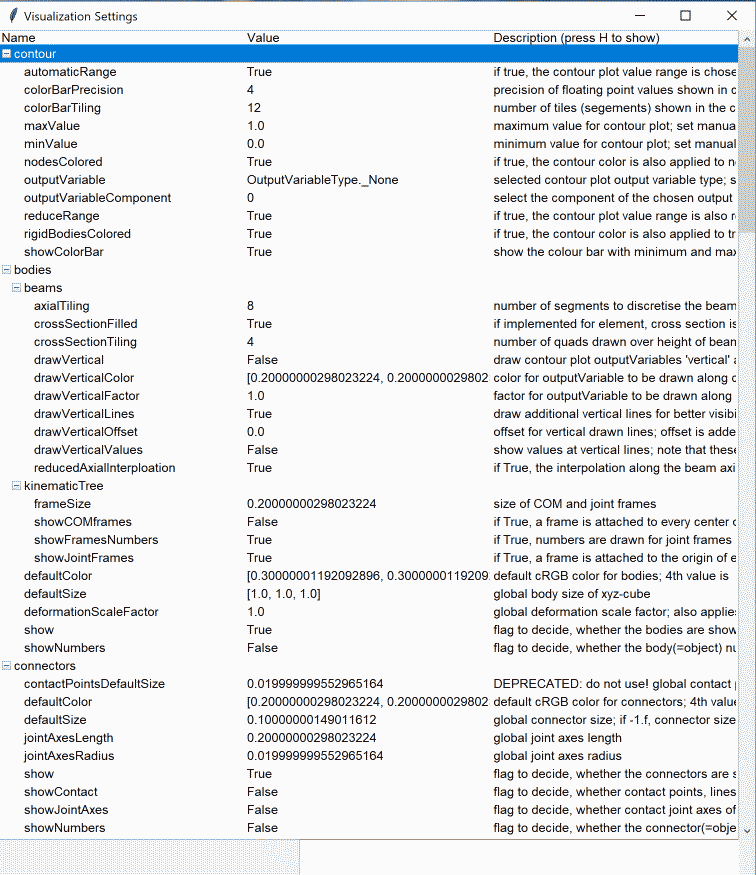
\includegraphics[width=0.8\columnwidth]{figures/visualizationSettings}
\end{center}
\caption{View of visualization settings (as of \codeName\ 1.5.51.dev1) (press 'V' in render window to open dialog)}%
\label{fig_visualizationSettings}%
\end{figure}
}

\noindent
The visualization settings structure can be accessed in the system container \texttt{SC} (access per reference, no copying!), accessing every value or structure directly, e.g.,
\pythonstyle\begin{lstlisting}
  SC.visualizationSettings.nodes.defaultSize = 0.001      #draw nodes very small

  #change openGL parameters; current values can be obtained from SC.GetRenderState()
  #change zoom factor:
  SC.visualizationSettings.openGL.initialZoom = 0.2       
  #set the center point of the scene (can be attached to moving object):
  SC.visualizationSettings.openGL.initialCenterPoint = [0.192, -0.0039,-0.075]

  #turn of auto-fit:
  SC.visualizationSettings.general.autoFitScene = False

  #change smoothness of a cylinder:
  SC.visualizationSettings.general.cylinderTiling = 100
  
  #make round objects flat:
  SC.visualizationSettings.openGL.shadeModelSmooth = False

  #turn on coloured plot, using y-component of displacements:
  SC.visualizationSettings.contour.outputVariable = exu.OutputVariableType.Displacement
  SC.visualizationSettings.contour.outputVariableComponent = 1 #0=x, 1=y, 2=z
\end{lstlisting}

\mysubsubsectionlabel{Renderer and 3D graphics}{sec:overview:basics:renderer}
A 3D renderer is attached to the simulation. Visualization is started with  \texttt{exu.StartRenderer()}, see the examples and tutorials.
The renderer uses an OpenGL window of a library called GLFW, which is platform-independent. 
The renderer is set up in a minimalistic way, just to ensure that you can check that the modeling is correct. There is no way to contruct models with the renderer. Try to avoid huge number of triangles in STL files or by creating large number of complex objects, such as spheres or cylinders.

\noindent There are some main features in the renderer, using keyboard and mouse:
\bi
  \item press key H to show help in renderer
  \item move model by pressing left mouse button and drag
  \item rotate model by pressing right mouse button and drag
  \item change visibility (wire frame, solid, transparent, ...) by pressing T
  \item zoom all: key A
  \item open visualization dialog: key V
  \item show item number: click on graphics element with left mouse button
  \item show item dictionary: click on graphics element with right mouse button  
  \item ... (see \refSection{sec:VSettingsGeneral}ff.)
\ei
%
Depending on your model (size, place, ...), you may need to adjust the following \texttt{openGL} parameters in \texttt{visualizationSettings}:
\bi
  \item light and light position 
  \item shadow (turned off by using 0; turned on by using, e.g., a value of 0.3) and shadow polygon offset; shadow slows down graphics performance by a factor of 2-3, depending on your graphics card
  \item visibility of nodes, markers, etc. in according bodies, nodes, markers, ..., \texttt{visualizationSettings}
  \item move camera with a selected marker: adjust \texttt{trackMarker} in \texttt{visualizationSettings.interactive}
  \item ... (see \refSection{sec:VSettingsGeneral}ff.)
\ei


\mysubsubsectionlabel{Graphics pipeline}{sec:overview:basics:graphicspipeline}
%deprecated, since there are user functions!: The user cannot interact with the visualization part for now.
There are basically two loops during simulation, which feed the graphics pipeline.
The solver runs a loop:
\bi
  \item compute step (or set up initial values)
  \item finish computation step; results are in current state
  \item copy current state to visualization state (thread safe)
  \item signal graphics pipeline that new visualization data is available
  \item the renderer may update the visualization depending on \texttt{graphicsUpdateInterval} in \\ \texttt{visualizationSettings.general}
\ei
The openGL graphics thread (=separate thread) runs the following loop:
\bi
  \item render openGL scene with a given graphicsData structure (containing lines, faces, text, ...)
  \item go idle for some milliseconds
  \item check if openGL rendering needs an update (e.g. due to user interaction)
  \item[] $\ra$ if update is needed, the visualization of all items is updated -- stored in a graphicsData structure)
  \item check if new visualization data is available and the time since last update is larger than a presribed value, the graphicsData structure is updated with the new visualization state
\ei

\mysubsubsectionlabel{Storing the model view}{sec:overview:basics:storingmodelview}
There is a simple way to store the current view (zoom, centerpoint, orientation, etc.) by using \texttt{SC.GetRenderState()} and \texttt{SC.SetRenderState()},
see also \refSection{sec:renderState}.
%
A simple way is to reload the stored render state (model view) after simulating your model once at the end of the simulation\footnote{
note that \texttt{visualizationSettings.general.autoFitScene} should be set False if you want to use the stored zoom factor}:
\pythonstyle\begin{lstlisting}
  import exudyn as exu
  SC=exu.SystemContainer()
  SC.visualizationSettings.general.autoFitScene = False #prevent from autozoom
  exu.StartRenderer()
  if 'renderState' in exu.sys:
      SC.SetRenderState(exu.sys['renderState']) 
  #+++++++++++++++
  #do simulation here and adjust model view settings with mouse
  #+++++++++++++++

  #store model view for next run:
  StopRenderer() #stores render state in exu.sys['renderState']
\end{lstlisting}
\horizontalRuler \\
%
Alternatively, you can obtain the current model view from the console after a simulation, e.g.,
\pythonstyle\begin{lstlisting}
  In[1] : SC.GetRenderState()
  Out[1]: 
  {'centerPoint': [1.0, 0.0, 0.0],
   'maxSceneSize': 2.0,
   'zoom': 1.0,
   'currentWindowSize': [1024, 768],
   'modelRotation': [[ 0.34202015,  0.        , 0.9396926 ],
                     [-0.60402274,  0.76604444, 0.21984631],
                     [-0.7198463 , -0.6427876 , 0.26200265]])}
\end{lstlisting}
%
which contains the last state of the renderer.
Now copy the output and set this with \texttt{SC.SetRenderState} in your Python code to have a fixed model view in every simulation (\texttt{SC.SetRenderState} AFTER \texttt{exu.StartRenderer()}):
\pythonstyle\begin{lstlisting}
  SC.visualizationSettings.general.autoFitScene = False #prevent from autozoom
  exu.StartRenderer()
  renderState={'centerPoint': [1.0, 0.0, 0.0],
               'maxSceneSize': 2.0,
               'zoom': 1.0,
               'currentWindowSize': [1024, 768],
               'modelRotation':     [[ 0.34202015,  0.        ,  0.9396926 ],
                                    [-0.60402274,  0.76604444,  0.21984631],
                                    [-0.7198463 , -0.6427876 ,  0.26200265]])
  SC.SetRenderState(renderState)
  #.... further code for simulation here
\end{lstlisting}
Note that in the current version of \codeName\ there is more data stored in render state, which is not used in \texttt{SC.SetRenderState},
see also \refSection{sec:renderState}.
\horizontalRuler
%

\mysubsubsection{Graphics user functions via Python}
There are some user functions in order to customize drawing:
\bi
  \item You can assign graphicsData to the visualization to most bodies, such as rigid bodies in order to change the shape. Graphics can also be imported from files (\texttt{GraphicsDataFromSTLfileTxt}) using the established format \ac{STL}\footnote{STereoLithography or Standard Triangle Language; file format available in nearly all CAD systems}.
  \item Some objects, e.g., \texttt{ObjectGenericODE2} or \texttt{ObjectRigidBody}, provide customized a function \texttt{graphicsDataUserFunction}. This user function just returns a list of GraphicsData, see \refSection{sec:graphicsData}. With this function you can change the shape of the body in every step of the computation.
  \item Specifically, the \texttt{graphicsDataUserFunction} in \texttt{ObjectGround} can be used to draw any moving background in the scene.
\ei
Note that all kinds of \texttt{graphicsDataUserFunction}s need to be called from the main (=computation) process as Python functions may not be called from separate threads (GIL). Therefore, the computation thread is interrupted to execute the \texttt{graphicsDataUserFunction} between two time steps, such that the graphics Python user function can be executed. There is a timeout variable for this interruption of the computation with a warning if scenes get too complicated.

\mysubsubsectionlabel{Color, RGBA and alpha-transparency}{sec:overview:basics:colorrgba}
Many functions and objects include color information. In order to allow alpha-transparency, all colors contain a list of 4 RGBA values, all values being in the range [0..1]:
\bi
  \item red (R) channel 
  \item green (G) channel  
  \item blue (B) channel 
  \item alpha (A) value, representing the so-called \mybold{alpha-transparency} (A=0: fully transparent, A=1: solid)
\ei
E.g., red color with no transparency is obtained by the color=[1,0,0,1]. Color predefinitions are found in \texttt{exudynGraphicsDataUtilities.py}, e.g., \texttt{color4red} or \texttt{color4steelblue} as well a list of 16 colors \texttt{color4list}, which is convenient to be used in a loop creating objects.

\mysubsubsectionlabel{Solution viewer}{sec:overview:basics:solutionviewer}
\codeName\ offers a convenient WYSIWYS -- 'What you See is What you Simulate' interface, showing you the computation results during simulation in the render window.
If you are running large models, it may be more convenient to watch results after simulation has been finished.
For this, you can use
\bi
  \item \texttt{interactive.SolutionViewer}, see \refSectionA{sec:interactive:SolutionViewer}
  \item \texttt{interactive.AnimateModes}, lets you view the animation of computed modes, see \refSectionA{sec:interactive:AnimateModes}
\ei
shown exemplary in \fig{fig_solutionViewer}.
\onlyRST{

.. _fig-solutionviewer:
.. figure:: docs/theDoc/figures/solutionViewer.png
   :width: 800

   View of \texttt{SolutionViewer} (as of \codeName\ 1.5.42.dev1)

}
\ignoreRST{
\begin{figure}[tbhp]%
\begin{center}
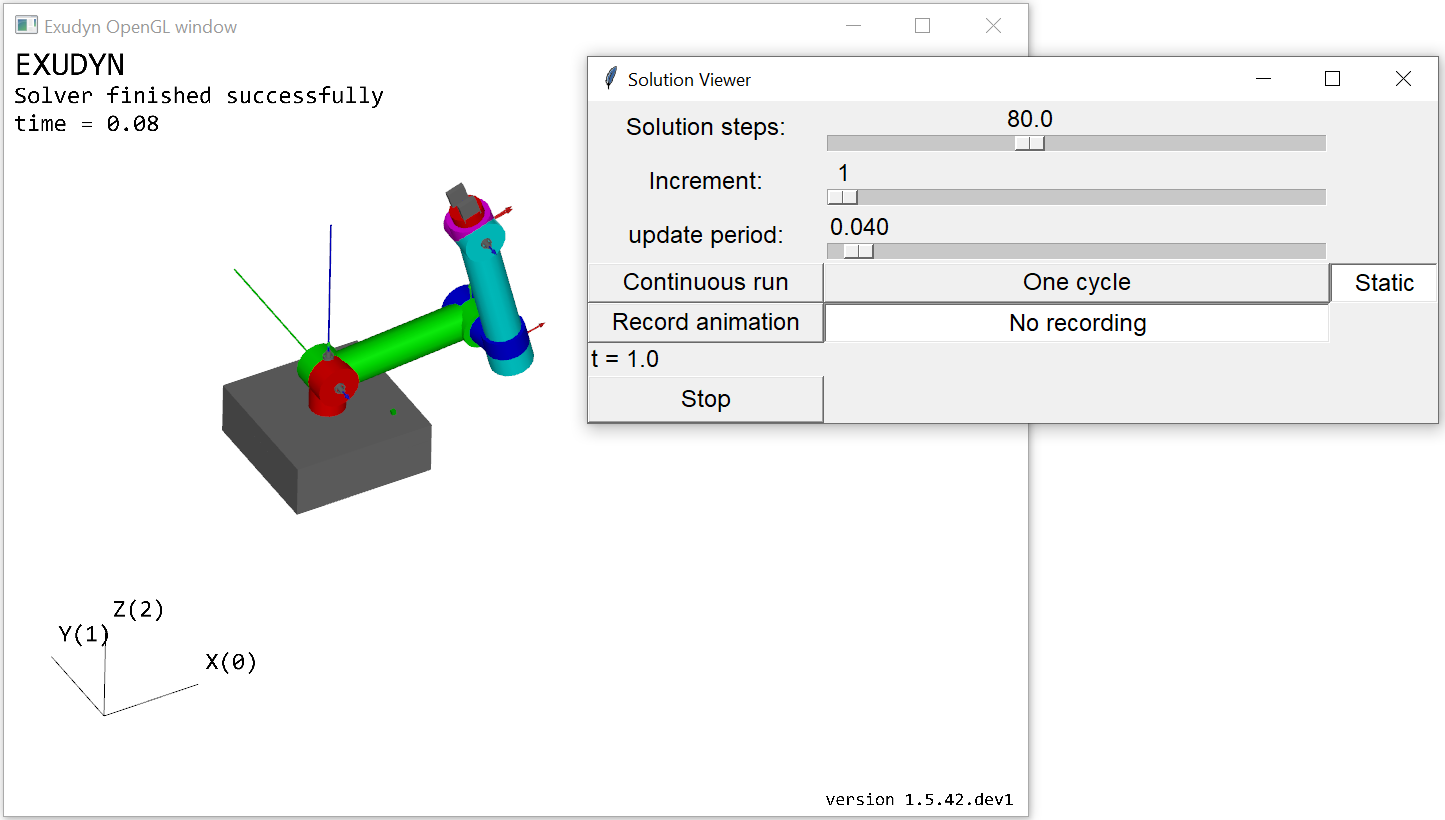
\includegraphics[width=0.98\columnwidth]{figures/solutionViewer}
\end{center}
\caption{View of \texttt{SolutionViewer} (as of \codeName\ 1.5.42.dev1)}%
\label{fig_solutionViewer}%
\end{figure}
}
The \texttt{SolutionViewer} adds a \texttt{tkinter} interactive dialog, which lets you interact with the model, with the following features:
\bi
\item The SolutionViewer represents a 'Player' for the dynamic solution or a series of static solutions, which is available after simulation if \texttt{solutionSettings.writeSolutionToFile = True}
\item The parameter \texttt{solutionSettings.solutionWritePeriod} represents the time period used to store solutions during dynamic computations.
\item As soon as 'Run' is pressed, the player runs (and it may be started automatically as well)
\item In the 'Static' mode, drag the slider 'Solution steps' to view the solution steps
\item In the 'Continuous run' mode, the player runs in an infinite loop
\item In the 'One cycle' mode, the player runs from the current position to the end; this is perfectly suited to record series of images for \mybold{creating animations}, see \refSection{sec:overview:basics:animations} and works together with the visualization settings dialog.
\ei
The solution should be loaded with
\texttt{LoadSolutionFile('coordinatesSolution.txt')}, where 'coordinatesSolution.txt' represents the stored solution file, 
see 
\bi
  \item \texttt{exu.SimulationSettings().solutionSettings.coordinatesSolutionFileName}
\ei
You can call the \texttt{SolutionViewer} either in the model, or at the command line / IPython to load a previous solution (belonging to the same mbs underlying the solution!):
\pythonstyle\begin{lstlisting}
  from exudyn.interactive import SolutionViewer
  sol = LoadSolutionFile('coordinatesSolution.txt')
  SolutionViewer(mbs, sol)
\end{lstlisting}
%
\mybold{Alternatively}, if no solution is provided, \texttt{SolutionViewer} tries to reload the solution of the previous simulation that is referred to from \texttt{mbs.sys$[$simulationSettings$]$}:
\pythonstyle\begin{lstlisting}
  from exudyn.interactive import SolutionViewer
  SolutionViewer(mbs)
\end{lstlisting}
An example for the \texttt{SolutionViewer} is integrated into the \texttt{Examples/} directory, see \texttt{solutionViewerTest.py}. \\
\mybold{Note}: The previous function \texttt{AnimateSolution} in \texttt{exudyn.utilities} allows to directly visualize the stored solution for according stored time frames without \texttt{tkinter} (useful for MacOS).

%+++++++++++++++++++++++++++++++++++++++++++++++++++++++++++++++++
\mysubsubsectionlabel{Generating animations}{sec:overview:basics:animations}
%
In many dynamics simulations, it is very helpful to create animations in order to better understand the motion of bodies. Specifically, the animation can be used to visualize the model much slower or faster than the model is computed.

Animations are created based on a series of images (frames, snapshots) taken during simulation. It is important, that the current view is used to record these images -- this means that the view should not be changed during the recording of images.
To turn on recording of images during solving, set the following flag to a positive value
\bi
  \item \texttt{simulationSettings.solutionSettings.recordImagesInterval = 0.01}
\ei
which means, that after every 0.01 seconds of simulation time, an image of the current view is taken and stored in the directory and filename (without filename ending) specified by 
\bi
  \item \texttt{SC.visualizationSettings.exportImages.saveImageFileName = "myFolder/frame"}
\ei
By default, a consecutive numbering is generated for the image, e.g., 'frame0000.png, frame0001.png,...'. Note that the standard file format PNG with ending '.png' uses compression libraries included in glfw, while the alternative TGA format produces '.tga' files which contain raw image data and therefore can become very large.

To create animation files, an external tool FFMPEG is used to efficiently convert a series of images into an animation.
\onlyRST{$\ra$ see theDoc.pdf !}
\ignoreRST{
In windows, simple DOS batch files can do the job to convert frames given in the local directory to animations, e.g.:
\plainlststyle
\lstinputlisting[breaklines=true, basicstyle=\ttm]{../userTools/makeAnimations/convertToVideo.bat}
After the video has been created, you should delete the single images:
\plainlststyle
\lstinputlisting[breaklines=true, basicstyle=\ttm]{../userTools/makeAnimations/deletePNGimages.bat}
}

%+++++++++++++++++++++++++++++++++++++++++++++++++++++++++++++++++
\mysubsubsectionlabel{Examples, test models and test suite}{sec:overview:basics:examplestestsuite}

The main collection of examples and models is available under
\bi
  \item \texttt{main/pythonDev/Examples}
  \item \texttt{main/pythonDev/TestModels}
\ei
You can use these examples to build up your own realistic models of multibody systems.
Very often, these models show the way which already works. Alternative ways may exist, but
sometimes there are limitations in the underlying C++ code, such that they won't work as you expect.

We would like to note that, even that some examples and test models contain comparison to 
papers of the literature or analytical solutions, there are many models which may not contain real
mechanical values and these models may not be converged in space or time 
(in order to keep running our test suite in less than a minute).

Finally, note that the \texttt{main/pythonDev/TestModels} are often only intended to preserve functionality
in the Python and C++ code (e.g., if global methods are changed), but they should not be misinterpreted as validation of the 
implemented methods. The \texttt{TestModels} are used in the \codeName\ \mybold{TestSuite} \texttt{TestModels/runTestSuite.py}
which is run after a full build of Python versions. Output for very version is written
to \texttt{main/pythonDev/TestSuiteLogs} containing the \codeName\ version and Python version. At the end of these
files, a summary is included to show if all models completed successfully (which means that a certain error level is achieved, which is rather small and different for the models).
There are also performance tests (e.g., if a certain implementation leads to a significant drop of performance).
However, the output of the performance tests is not stored on github.

We are trying hard to achieve error-free algorithms of physically correct models, but there may always be some errors in the code.

%+++++++++++++++++++++++++++++++++++++++++++++++++++++++++++++++++
\mysubsubsectionlabel{Removing convergence problems and solver failures}{sec:overview:basics:convergenceproblems}
Nonlinear formulations (such as most multibody systems, especially nonlinear finite elements) cause problems and there is no general nonlinear solver which may reliably and accurately solve such problems.
Tuning solver parameters is at hand of the user. 
In general, the Newton solver tries to reduce the error by the factor given in \texttt{simulationSettings.staticSolver.newton.relativeTolerance} (for static solver), which is not possible for very small (or zero) initial residuals. The absolute tolerance is helping out as a lower bound for the error, given in \texttt{simulationSettings.staticSolver.newton.absoluteTolerance} (for static solver), which is by default rather low (1e-10) -- in order to achieve accurate results for small systems or small motion (in mm or $\mu$m regime). Increasing this value helps to solve such problems. Nevertheless, you should usually set tolerances as low as possible because otherwise, your solution may become inaccurate.

\noindent The following hints shall be followed (also some solver hints).
\bi
  \item \mybold{static solver}: load steps are reduced even if the solution seems to be smooth and less steps are expected; larger number of steps may happen for finer discretization; you may adjust (increase) \texttt{.newton.relativeTolerance} / \texttt{.newton.absoluteTolerance} in static solver or in time integration to resolve such problems, but check if solution achieves according accuracy
  \item \mybold{static solver}: load steps are reduced significantly for highly nonlinear problems; solver repeatedly writes that steps are reduced $\ra$ try to use \texttt{loadStepGeometric} and use a large \texttt{loadStepGeometricRange}: this allows to start with very small loads in which the system is nearly linear (e.g. for thin strings or belts under gravity).
  \item \mybold{static solver}: in case that your system is (nearly) kinematic, a static solution can be achieved using \texttt{stabilizerODE2term}, which adds mass-proportional stiffness terms during load steps $< 1$.
  \item very small loads or even \mybold{zero loads} do not converge: \texttt{SolveDynamic} or \texttt{SolveStatic} \mybold{terminated due to errors}
  \bi
  \item[$\ra$] the reason is the nonlinearity of formulations (nonlinear kinematics, nonlinear beam, etc.) and round off errors, which restrict Newton to achieve desired tolerances
  \item[$\ra$] adjust (increase) \texttt{.newton.relativeTolerance} / \texttt{.newton.absoluteTolerance} in static solver or in time integration
  \item[$\ra$] in many cases, especially for static problems, the \texttt{.newton.newtonResidualMode = 1} evaluates the increments; the nonlinear problems is assumed to be converged, if increments are within given absolute/relative tolerances; this also works usually better for kinematic solutions
  \ei
  \item for \mybold{discontinuous problems}: try to adjust solver parameters; especially the \texttt{discontinuous.iterationTolerance} and \texttt{discontinuous.maxIterations}; try to make smaller load or time steps in order to resolve switching points of contact or friction; generalized alpha solvers may cause troubles when reducing step sizes $\ra$ use TrapezoidalIndex2 solver
  \item if you see further problems, please post them (including relevant example) at the \codeName\ github page!
\ei

%+++++++++++++++++++++++++++++++++++++++++++++++++++++++++++++++++
\mysubsubsectionlabel{Performance and ways to speed up computations}{sec:overview:basics:speedup}
%
Multibody dynamics simulation should be accurate and reliable on the one hand side. Most solver settings are such that they lead to comparatively reliable results.
However, in some cases there is a significant possibility for speeding up computations, which are described in the following list. Not all recommendations may apply to your models.

The following examples refer to \texttt{simulationSettings = exu.SimulationSettings()}.
In general, to see where CPU time is lost, use the option turn on \texttt{simulationSettings.displayComputationTime = True} to see which parts of the solver need most of the time (deactivated in exudynFast versions!).

To activate the \codeName\ C++ versions without range checks, which may be approx.\ 30 percent faster in some situations, use the following code snippet before first import of \texttt{exudyn}:
\pythonstyle\begin{lstlisting}
  import sys
  sys.exudynFast = True #this variable is used to signal to load the fast exudyn module
  import exudyn as exu
\end{lstlisting}
The faster versions are available for all release versions, but only for some \texttt{.dev1} development versions (Python 3.10), which can be determined by trying \texttt{import exudyn.exudynCPPfast}.

\noindent However, there are many \mybold{ways to speed up \codeName\ in general}:
\bi
  \item for models with more than 50 coordinates, switching to sparse solvers might greatly improve speed: \texttt{simulationSettings.linearSolverType = exu.LinearSolverType.EigenSparse}
  \item try to avoid Python functions or try to speed up Python functions
  \item instead of user functions in objects or loads (computed in every iteration), some problems would also work if these parameters are only updated in \texttt{mbs.SetPreStepUserFunction(...)}
  \item Python user functions can be speed up using the Python numba package, using \texttt{@jit} in front of functions (for more options, see \exuUrl{https://numba.pydata.org/numba-doc/dev/user/index.html}{https://numba.pydata.org/numba-doc/dev/user/index.html}); Example given in \texttt{Examples/springDamperUserFunctionNumbaJIT.py} showing speedups of factor 4; more complicated Python functions may see speedups of 10 - 50
  %
  \item for \mybold{discontinuous problems}, try to adjust solver parameters; especially the discontinuous.iterationTolerance which may be too tight and cause many iterations; iterations may be limited by discontinuous.maxIterations, which at larger values solely multiplies the computation time with a factor if all iterations are performed
  \item For multiple computations / multiple runs of Exudyn (parameter variation, optimization, compute sensitivities), you can use the processing sub module of \codeName\ to parallelize computations and achieve speedups proporional to the number of cores/threads of your computer; specifically using the \texttt{multiThreading} option or even using a cluster (using \texttt{dispy}, see \texttt{ParameterVariation(...)} function)
  \item In case of multiprocessing and cluster computing, you may see a very high CPU usage of "Antimalware Service Executable", which is the Microsoft Defender Antivirus; you can turn off such problems by excluding \texttt{python.exe} from the defender (on your own risk!) in your settings:\\
  %
  Settings $\ra$ Update \& Security $\ra$ Windows Security $\ra$ Virus \& threat protection settings $\ra$ Manage settings $\ra$ Exclusions $\ra$ Add or remove exclusions 
\ei
%
\mybold{Possible speed ups for dynamic simulations}:
\bi
  \item for implicit integration, turn on \mybold{modified Newton}, which updates jacobians only if needed: \texttt{simulationSettings.timeIntegration.newton.useModifiedNewton = True}
  \item use \mybold{multi-threading}: \texttt{simulationSettings.parallel.numberOfThreads = ...}, depending on the number of cores (larger values usually do not help); improves greatly for contact problems, but also for some objects computed in parallel; will improve significantly in future
  \item decrease number of steps (\texttt{simulationSettings.timeIntegration.numberOfSteps = int(tEnd/h)}) by increasing the step size $h$ if not needed for accuracy reasons; not that in general, the solver will reduce steps in case of divergence, but not for accuracy reasons, which may still lead to divergence if step sizes are too large
  \item switch off measuring computation time, if not needed: \texttt{simulationSettings.displayComputationTime = False}
  \item try to switch to \mybold{explicit solvers}, if problem has no constraints and if problem is not stiff
  \item try to have \mybold{constant mass matrices} (see according objects, which have constant mass matrices; e.g. rigid bodies using RotationVector Lie group node have constant mass matrix)
  \item for explicit integration, set \texttt{computeEndOfStepAccelerations = False}, if you do not need accurate evaluation of accelerations at end of time step (will then be taken from beginning)
  \item for explicit integration, set \texttt{explicitIntegration.computeMassMatrixInversePerBody=True}, which avoids factorization and back substitution, which may speed up computations with many bodies / particles
  \item if you are sure that your mass matrix is constant, set \texttt{simulationSettings.timeIntegration.reuseConstantMassMatrix = True}; check results!
  \item check that \texttt{simulationSettings.timeIntegration.simulateInRealtime = False}; if set True, it breaks down simulation to real time
  \item do not record images, if not needed: \texttt{simulationSettings.solutionSettings.recordImagesInterval = -1}
  \item in case of bad convergence, decreasing the step size might also help; check also other flags for adaptive step size and for Newton
  \item use \texttt{simulationSettings.timeIntegration.verboseMode = 1}; larger values create lots of output which drastically slows down
  \item use \texttt{simulationSettings.timeIntegration.verboseModeFile = 0}, otherwise output written to file
  \item adjust \texttt{simulationSettings.solutionSettings.sensorsWritePeriod} to avoid time spent on writing sensor files
  \item use \texttt{simulationSettings.timeIntegration.writeSolutionToFile = False}, otherwise much output may be written to file; 
  \item if solution file is needed, adjust \texttt{simulationSettings.solutionSettings.solutionWritePeriod} to larger values and also adjust \texttt{simulationSettings.solutionSettings.outputPrecision}, e.g., to 6, in order to avoid larger files; also adjust \texttt{simulationSettings.solutionSettings.exportVelocities = False} and \texttt{simulationSettings.solutionSettings.exportAccelerations = False} to avoid large output files
\ei


%+++++++++++++++++++++++++++++++++++++++++++++++++++++++++++++++++
%+++++++++++++++++++++++++++++++++++++++++++++++++++++++++++++++++
\mysubsectionlabel{Advanced topics}{sec:overview:advanced}
%
This section covers some advanced topics, which may be only relevant for a smaller group of people. 
Functionality may be extended but also removed in future
%
\mysubsubsectionlabel{Camera following objects and interacting with model view}{sec:overview:advanced:camerafollowing}
%
For some models, it may be advantageous to track the translation and/or rotation of certain bodies, e.g., for cars, (wheeled) robots or bicycles. 
To do so, the current render state (\texttt{SC.GetRenderState()}, \texttt{SC.SetRenderState(...)}) can be obtained and modified, in order to always follow a certain position.
As this needs to be done during redraw of every frame, it is conveniently done in a graphicsUserFunction, e.g., within the ground body. This is shown in the following example, in which \texttt{mbs.variables['nTrackNode']} is a node number to be tracked:
%
\pythonstyle\begin{lstlisting}
  #mbs.variables['nTrackNode'] contains node number
  def UFgraphics(mbs, objectNum):
      n = mbs.variables['nTrackNode']
      p = mbs.GetNodeOutput(n,exu.OutputVariableType.Position, 
                            configuration=exu.ConfigurationType.Visualization)
      rs=SC.GetRenderState() #get current render state
      A = np.array(rs['modelRotation'])
      p = A.T @ p #transform point into model view coordinates
      rs['centerPoint']=[p[0],p[1],p[2]]
      SC.SetRenderState(rs)  #modify render state
      return []

  #add object with graphics user function
  oGround2 = mbs.AddObject(ObjectGround(visualization=
                 VObjectGround(graphicsDataUserFunction=UFgraphics)))
  #.... further code for simulation here
\end{lstlisting}
%
%+++++++++++++++++++++++++++++++++++++++++++++++++++++++++++++++++
%+++++++++++++++++++++++++++++++++++++++++++++++++++++++++++++++++
\mysubsubsectionlabel{Contact problems}{sec:overview:advanced:contact}
%
Since Q4 2021 a contact module is available in \codeName. 
This separate module \texttt{GeneralContact} $[$\mybold{still under development, consider with care!}$]$ is highly optimized and implemented with parallelization (multi-threaded) for certain types of contact elements.
\onlyRST{

.. _fig-contactexamples:
.. figure:: docs/theDoc/figures/contactTests.png
   :width: 450
   
.. figure:: docs/theDoc/figures/contactTests2.jpg
   :width: 450
  
   Some tests and examples using \texttt{GeneralContact}

}
%.. |cpic1| image:: docs/theDoc/figures/
%   :width: 45%
%
%.. |cpic2| image:: docs/theDoc/figures/contactTests2.jpg
%   :width: 45%
%
%|cpic1| |cpic2|
%
%[Some tests and examples using \texttt{GeneralContact}]

\ignoreRST{
\begin{figure}[tbh]%
\begin{center}
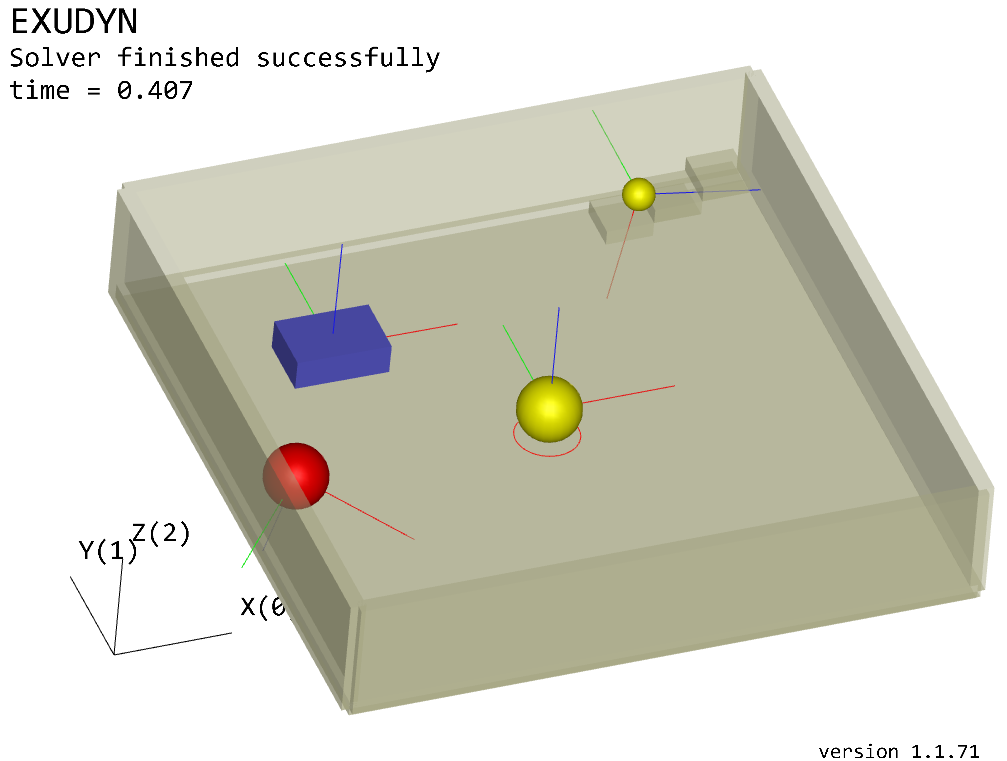
\includegraphics[width=0.35\columnwidth]{figures/contactTests} \hspace{1cm}%
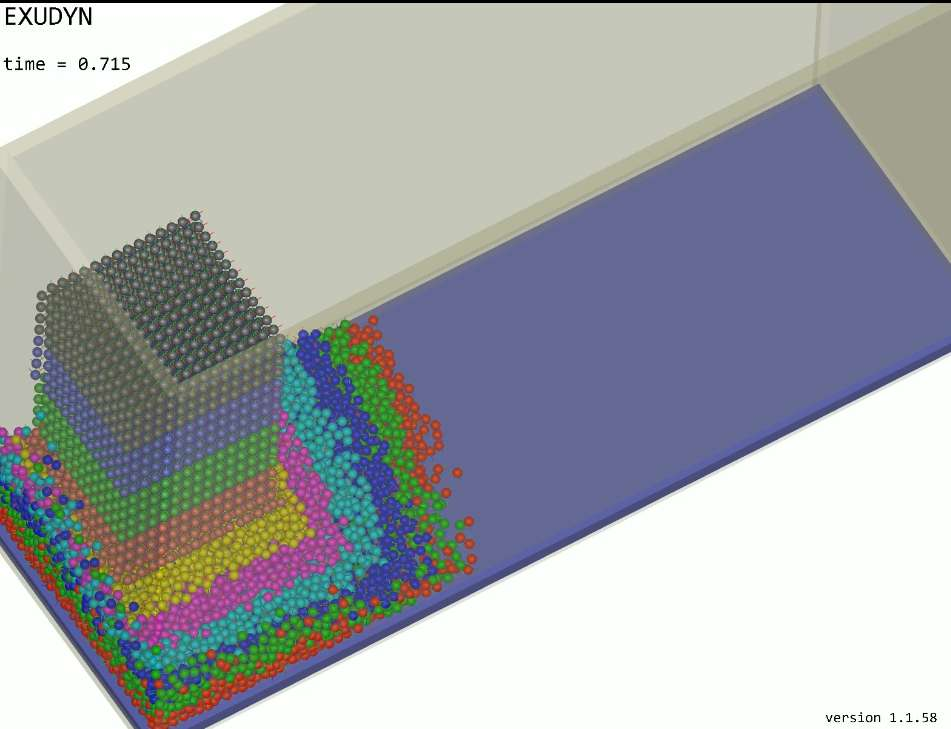
\includegraphics[width=0.35\columnwidth]{figures/contactTests2}%
\end{center}
\caption{Some tests and examples using \texttt{GeneralContact}.}%
\label{fig:contactExamples}%
\end{figure}
}

\noindent \mybold{Note}:
\bi
\item \texttt{GeneralContact} is (in most cases) restricted to dynamic simulation (explicit or implicit $[$\mybold{still under development, consider with care!}$]$) if friction is used; without friction, it also works in the static case
\item in addition to \texttt{GeneralContact} there are special objects, in particular for rolling and simple 1D contacts, that are available as single objects, cf.\ \texttt{ObjectConnectorRollingDiscPenalty}
\item \texttt{GeneralContact} is recommended to be used for large numbers of contacts, while the single objects are integrated more directly into mbs.
\ei

\noindent Currently, \texttt{GeneralContact} includes:
\bi
  \item Sphere-Sphere contact (attached to any marker); may represent circle-circle contact in 2D
  \item Triangles mounted on rigid bodies, in contact with Spheres [only explicit]
  \item ANCFCable2D contacting with spheres (which then represent circles in 2D) [partially implicit, needs revision]
\ei
For details on the contact formulations, see \refSection{secContactTheory}.

%+++++++++++++++++++++++++++++++++++++++++++++++++++++++++++++++++
%+++++++++++++++++++++++++++++++++++++++++++++++++++++++++++++++++
\mysubsubsectionlabel{OpenVR}{sec:overview:advanced:openvr}
%
The general open source libraries from Valve, see
\bi
\item[] https://github.com/ValveSoftware/openvr
\ei
have been linked to \codeName\ . In order to get OpenVR fully integrated, you need to run \texttt{setup.py} \codeName\ with the \texttt{--openvr} flag. For general installation instructions, see \refSection{sec:install:installinstructions}.

Running OpenVR either requires an according head mounted display (HMD) or a virtualization using, e.g., Riftcat 2 to use a mobile phone with an according adapter. Visualization settings are available in \texttt{interactive.openVR}, but need to be considered with care.
An example is provided in \texttt{openVRengine.py}, showing some optimal flags like locking the model rotation, zoom or translation.

Everything is experimental, but contributions are welcome!

%+++++++++++++++++++++++++++++++++++++++++++++++++++++++++++++++++
%+++++++++++++++++++++++++++++++++++++++++++++++++++++++++++++++++
\mysubsubsectionlabel{Interaction with other codes}{sec:overview:advanced:interactwithcodes}
%
Interaction with other codes and computers (E.g., MATLAB or other C++ codes, or other Python versions)
is possible. 
To connect to any other code, it is convenient to use a TCP/IP connection. This is enabled via 
the \texttt{exudyn.utilities} functions
\bi
\item \texttt{CreateTCPIPconnection}
\item \texttt{TCPIPsendReceive}
\item \texttt{CloseTCPIPconnection}
\ei
Basically, data can be transmitted in both directions, e.g., within a preStepUserFunction. In Examples, you can find 
 TCPIPexudynMatlab.py which shows a basic example for such a connectivity.

%+++++++++++++++++++++++++++++++++++++++++++++++++++++++++++++++++
%+++++++++++++++++++++++++++++++++++++++++++++++++++++++++++++++++
\mysubsubsectionlabel{ROS}{sec:overview:advanced:ros}
%
Basic interaction with ROS has been tested. However, make sure to use Python 3, as there is no (and will never be any) Python 2
support for \codeName\ .





%+++++++++++++++++++++++++++++++++++++++++++++++++++++++++++++++++++++++++++++++
%+++++++++++++++++++++++++++++++++++++++++++++++++++++++++++++++++++++++++++++++

\mysubsectionlabel{C++ Code}{sec:overview:cppcode}
This section covers some information on the C++ code. For more information see the Open source code and use doxygen.

Exudyn was developed for the efficient simulation of flexible multi-body systems. Exudyn was designed for rapid implementation and testing of new formulations and algorithms in multibody systems, whereby these algorithms can be easily implemented in efficient C++ code. The code is applied to industry-related research projects and applications.

\mysubsubsection{Focus of the C++ code}
The code focuses on four principles, starting with highest priority: 
\bn
  \item developer-friendly
  \item error minimization
  \item user-friendliness
  \item efficiency
\en
The focus is therefore on:
\bi
    \item A developer-friendly basic structure regarding the C++ class library and the possibility to add new components.
    \item The basic libraries are slim, but extensively tested; only the necessary components are available
    \item Complete unit tests are added to new program parts during development; for more complex processes, tests are available in Python
    \item In order to implement the sometimes difficult formulations and algorithms without errors, error avoidance is always prioritized.
    \item To generate efficient code, classes for parallelization (vectorization and multithreading) are provided. We live the principle that parallelization takes place on multi-core processors with a central main memory, and thus an increase in efficiency through parallelization is only possible with small systems, as long as the program runs largely in the cache of the processor cores. Vectorization is tailored to SIMD commands as they have Intel processors, but could also be extended to GPGPUs in the future.
    \item The user interface (Python) provides a nearly 1:1 image of the system and the processes running in it, which can be controlled with the extensive possibilities of Python.
\ei

\mysubsubsection{C++ Code structure}
%
The following \mybold{entry points} into the C++ code can be found:
\bi
  \item Python -- C++: the creation of the module \texttt{exudyn} is found in:\\
  
  \texttt{main/src/Pymodules/PybindModule.cpp}\\
  it includes large header files, which are automatically created for binding C++ code with Python.%blank line needed for .rst:
  
  \item The object factory for creation of items (calling \texttt{mbs.AddNode(...)} and similar): \\
    \texttt{main/src/Main/MainObjectFactory.h / .cpp}
  \item Using the VisualStudio \texttt{.sln} file and using the Debug mode allows you to smoothly walk from Python to C++ code (though that this takes some time to start up and it does not work always; and it does not work for graphics if it runs in a separate thread).
\ei

The functionality of the code is mainly based on systems (MainSystem and CSystem), items and solvers representing the multibody system or similar physical systems to be simulated. Parts of the core structure of Exudyn are:
\bi
  \item CSystem / MainSystem: a multibody system which consists of nodes, objects, markers, loads, etc.
  \item SystemContainer: holds a set of systems; connects to visualization (container)
  \item items: node, (computational) object, marker, load, sensor
  \item computational objects: efficient objects for computation = bodies, connectors, connectors, loads, nodes, ...
  \item visualization objects: interface between computational objects and 3D graphics
  \item main (manager) objects: do all tasks (e.g. interface to visualization objects, GUI, Python, ...) which are not needed during computation
  \item static solver, kinematic solver, time integration
  \item Python interface via pybind11; items are accessed with a dictionary interface; system structures and settings read/written by direct access to the structure (e.g. SimulationSettings, VisualizationSettings)
  \item interfaces to linear solvers; future: optimizer, eigenvalue solver, ... (mostly external or in Python)
  \item \mybold{autogenerated}: this folder in \texttt{main/src} contains many item definitions as well as other interface files; they are all automatically generated by some Python code and should not be changed manually as they will be overwritten.
\ei


\mysubsubsection{C++ Code: Modules}
The following internal modules are used, which are represented by directories in \texttt{main/src}:
\bi
  \item Autogenerated: item (nodes, objects, markers and loads) classes split into main (management, Python connection), visualization and computation
  \item Graphics: a general data structure for 2D and 3D graphical objects and a tiny openGL visualization; linkage to GLFW
    \item Linalg: Linear algebra with vectors and matrices; separate classes for small vectors (SlimVector), large vectors (Vector and ResizableVector), vectors without copying data (LinkedDataVector), and vectors with constant size (ConstVector)
  \item Main: mainly contains SystemContainer, System and ObjectFactory
  \item Objects: contains the implementation part of the autogenerated items
  \item Pymodules: manually created libraries for linkage to Python via pybind; remaining linking to Python is located in autogenerated folder
  \item pythonGenerator: contains Python files for automatic generation of C++ interfaces and Python interfaces of items;
  \item Solver: contains all solvers for solving a CSystem
  \item System: contains core item files (e.g., MainNode, CNode, MainObject, CObject, ...)
  \item Tests: files for testing of internal linalg (vector/matrix), data structure libraries (array, etc.) and functions
    \item Utilities: array structures for administrative/managing tasks (indexes of objects ... bodies, forces, connectors, ...); basic classes with templates and definitions
\ei

The following main external libraries are linked to Exudyn:
\bi
  \item LEST: for testing of internal functions (e.g. linalg)
  \item GLFW: 3D graphics with openGL; cross-platform capabilities
  \item Eigen: linear algebra for large matrices, linear solvers, sparse matrices and link to special solvers
  \item pybind11: linking of C++ to Python
\ei

\mysubsubsection{Code style and conventions}
%
This section provides general coding rules and conventions, partly applicable to the C++ and Python parts of the code. Many rules follow common conventions (e.g., google code style, but not always -- see notation):
\bi
    \item write simple code (no complicated structures or uncommon coding)
    \item write readable code (e.g., variables and functions with names that represent the content or functionality; AVOID abbreviations)
    \item put a header in every file, according to Doxygen format
    \item put a comment to every (global) function, member function, data member, template parameter
    \item ALWAYS USE curly brackets for single statements in 'if', 'for', etc.; example: if (i<n) \{i += 1;\}
    \item use Doxygen-style comments (use '//!' Qt style and '@ date' with '@' instead of '\' for commands)
    \item use Doxygen (with preceeding '@') 'test' for tests, 'todo' for todos and 'bug' for bugs
    \item USE 4-spaces-tab
    \item use C++11 standards when appropriate, but not exhaustively
    \item ONE class ONE file rule (except for some collectors of single implementation functions)
    \item add complete unit test to every function (every file has link to LEST library)
    \item avoid large classes (>30 member functions; > 15 data members)
    \item split up god classes (>60 member functions)
    \item mark changed code with your name and date
    \item REPLACE tabs by spaces: Extras->Options->C/C++->Tabstopps: tab stopp size = 4 (=standard) +  KEEP SPACES=YES
\ei

\mysubsubsection{Notation conventions}
%
The following notation conventions are applied (\mybold{no exceptions!}):
\bi
    \item use lowerCamelCase for names of variables (including class member variables), consts, c-define variables, ...; EXCEPTION: for algorithms following formulas, e.g., $f = M*q_{tt} + K*q$, GBar, ...
    \item use UpperCamelCase for functions, classes, structs, ...
    \item Special cases for CamelCase (with some exceptions that happened in the past ...): 
    \bi
    \item continue upper case after upper case abbreviations in case of \mybold{functions or classes}: 'ODESystem', 'Point2DClass', 'ANCFCable2D', 'ANCFALE', 'ComputeODE1Equations', ... (this is not always nice to read, but has become a standard and will be further used!) 
    \item for variables and class member variables continue \mybold{lower case}: 'nODE1variables', 'dim2Dspecial', 'ANCFsize'
    \item abbreviations at beginning of expressions: for functions or classes use \texttt{ODEComputeCoords()}, for variables avoid 'ODE' at beginning: use 'nODE' or write 'odeCoordinates'
    \ei
    \item '[...]Init' ... in arguments, for initialization of variables; e.g. 'valueInit' for initialization of member variable 'value'
    \item use American English throughout: Visualization, etc.
    \item AVOID consecutive capitalized words, e.g., avoid 'ODEAE'
    \item do not use '\_' within variable or function names; exception: derivatives
    \item use name which exactly describes the function/variable: 'numberOfItems' instead of 'size' or 'l'
    \item examples for variable names: secondOrderSize, massMatrix, mThetaTheta
    \item examples for function/class names: \texttt{SecondOrderSize}, \texttt{EvaluateMassMatrix}, \texttt{Position(const Vector3D\& localPosition)}
    \item use the Get/Set...() convention if data is retrieved from a class (Get) or something is set in a class (Set); Use \texttt{const T\& Get()/T\& Get} if direct access to variables is needed; Use Get/Set for pybind11
    \item example Get/Set: \texttt{Real* GetDataPointer()}, \texttt{Vector::SetAll(Real)}, \texttt{GetTransposed()}, \texttt{SetRotationalParameters(...)}, \texttt{SetColor(...)}, ...
    \item use 'Real' instead of double or float: for compatibility, also for AVX with SP/DP
    \item use 'Index' for array/vector size and index instead of size\_t or int
    \item item: object, node, marker, load: anything handled within the computational/visualization systems
    \item Do not use numbers (3 for 3D or any other number which represents, e.g., the number of rotation parameters). Use const Index or constexpr to define constants.
\ei

\mysubsubsection{No-abbreviations-rule}
%
The code uses a \mybold{minimum set of abbreviations}; however, the following abbreviation rules are used throughout:
In general: DO NOT ABBREVIATE function, class or variable names: GetDataPointer() instead of GetPtr(); exception: cnt, i, j, k, x or v in cases where it is really clear (short, 5-line member functions).

\mybold{Exceptions} to the NO-ABBREVIATIONS-RULE, see also \hyperref[sec:listOfAbbreviations]{\underline{List of Abbreviations}}: %no section number!!!: \refSection{sec:listOfAbbreviations}
\bi
    \item \ac{ODE}
    \item \ac{ODE2}: marks parts related to second order differential equations (SOS2, EvalF2 in HOTINT)
    \item \ac{ODE1}: marks parts related to first order differential equations (ES, EvalF in HOTINT)
    \item \ac{AE}; note: using the term 'AEcoordinates' for 'algebraicEquationsCoordinates'
    \item 'C[...]' ... Computational, e.g. for ComputationalNode ==> use 'CNode'
    \item \ac{mbs}
    \item \ac{min}, \ac{max}
    \item \ac{abs}, \ac{rel}
    \item \ac{trig} 
    \item \ac{quad}
    \item \ac{RHS}
    \item \ac{LHS}
    \item \ac{EP}
    \item \ac{Rxyz}%: consecutive rotations around x, y and z-axis (Tait-Bryan rotations);
    \item \ac{coeffs}
    \item \ac{pos}
    \item \ac{T66}; based on $6\times 6$ matrix transformations
    \item write time derivatives with underscore: \_t, \_tt; example: Position\_t, Position\_tt, ...
    \item write space-wise derivatives ith underscore: \_x, \_xx, \_y, ...
    \item if a scalar, write coordinate derivative with underscore: \_q, \_v (derivative w.r.t. velocity coordinates)
    \item for components, elements or entries of vectors, arrays, matrices: use 'item' throughout
    \item '[...]Init' ... in arguments, for initialization of variables; e.g. 'valueInit' for initialization of member variable 'value'
\ei

%+++++++++++++++++++++++++++++++++++++++++++++++++++++++++++++++++++++++++++++++
%+++++++++++++++++++++++++++++++++++++++++++++++++++++++++++++++++++++++++++++++

\mysubsubsection{Implementation of new computational items in C++}
%
This section should sketch which changes will be needed to integrate new C++ items.
In general, it is recommended to first start with a Python implementation with user functions based on
\texttt{NodeGeneric...}, \texttt{ObjectGeneric...}, \texttt{ObjectConnectorCoordinateVector} for constraints and
any suitable connector for new nodes or objects. New sensors can be based on the \texttt{SensorUserFunction}.

If such an implementation is successful, but too slow, a C++ implementation can be considered.
In the following, two use cases are shown, which show the simplicity of the procedure:
\bi
  \item \mybold{Case 1}: user object (body):\\
  %
  It is recommended to first search for a body with a similar behavior.
  Copy the definition of such an object inside the file \texttt{objectDefinition.py} and edit the according lines. 
  There is not much description of 
  this file yet (except from the first lines of the file), as it will be transformed into another format in the future.
  Basically, you need to edit the interface, which contains parameters (which are linked to Python) and functions, 
  which go to the header file.
  When you finished editing, run \texttt{pythonAutoGenerateObjects.py}. This generates the header file in \texttt{src/autogenerated}
  but also adds description to some docs files and adds the \texttt{pybind11} interface. 
  Now copy the implementation (\texttt{.cpp}) file of the same connector from which you copied from and rename and edit all functions.
  %
  For the body
  \bi
    \item \texttt{ComputeMassMatrix}: computes the mass matrix either in sparse or dense mode; this function is performance-critical if the mass matrix is non-constant
    \item \texttt{ComputeODE2LHS}: computes the \ac{LHS} generalized forces of the body; this function is performance-critical
    \item \texttt{GetAccessFunctionTypes}: specifies, which access functions are available in \texttt{GetAccessFunctionBody(...)}
    \item \texttt{GetAccessFunctionBody}: needs to compute functions for 'access' to the body, in the sense that e.g.\ forces or torques can be applied. 
    \item \texttt{GetAvailableJacobians}: shall return the flags which jacobians of \texttt{ComputeODE2LHS} need to be computed and which are available as functions; binary flags added up
    \item \texttt{GetOutputVariableBody}: function needs to implement the output variables, such as position, acceleration, forces, etc.\ as defined in \texttt{GetOutputVariableTypes()}
    \item \texttt{HasConstantMassMatrix}: specifies, if mass matrix is constant
    \item \texttt{GetNumberOfNodes}: number of nodes of object
    \item \texttt{GetODE2Size}: total number of \ac{ODE2} coordinates
    \item \texttt{GetType}: some flags for objects, such as \texttt{Body}, \texttt{SingleNoded}, \texttt{SuperElement}, ...; these flags are needed for connectivity and special treatment in the system
    \item \texttt{GetPosition, GetVelocity, ...}: provide this functions as far as possible; rigid bodies need to provide positions and rotation matrix, as well as velocity and angular velocity for markers; if functions do not exist, some marker or sensor functions may fail
    \item ...   possibly some helper functions, which you should implement for the functionality of your object.
  \ei
  \item \mybold{Case 2}: user connector:\\
  It is recommended to search for a connector with similar behavior; first check, if you would like to implement 
  an algebraic constraint or a spring-damper-like connector.
  Again, copy a similar connector in \texttt{objectDefinition.py} and edit the according lines. 
  When you finished editing, run \texttt{pythonAutoGenerateObjects.py} and make a copy of the copied implementation (\texttt{.cpp}) file.
  The implementation file usually consists of
  \bi
    \item \texttt{ComputeODE2LHS}: this function shall compute the \ac{LHS} generalized forces on the two marker objects
    \item \texttt{ComputeJacobianODE2\_ODE2}: computes the \texttt{GetAvailableJacobians()} is not providing any '...\_function' flag, which indicates that these jacobians are available as function
    \item \texttt{GetOutputVariableConnector}: this function needs to compute all output variables as given in \texttt{GetOutputVariableTypes()}
    \item ...   possibly some helper functions, which you should implement for the functionality of your object.
  \ei
\ei



%+++++++++++++++++++++++++++++++++++++++++++++++++++++++++++++++++++++++++++++++
%+++++++++++++++++++++++++++++++++++++++++++++++++++++++++++++++++++++++++++++++

%\ignoreRST{
%\mysubsection{Changes}
%\label{sec:changes}
%For continuous tracking of changes, see \refSection{sec:issueTracker}.
%}
